\documentclass{foils}

%\newfont{\cmrhuge}{cmr17 at 160.8pt}
\newfont{\cmrhuge}{cmss17 at 160.8pt}
%\newfont{\cmrhuge2}{cmss17 at 100.8pt}

\topmargin=-65pt
\textheight=7in
\textwidth=10.5in
%%\headsep=.25in
%%\headheight=0in
\oddsidemargin=-.75in
\evensidemargin=-.75in
\usepackage{color}
\usepackage{epsfig}
\usepackage{graphicx}
\special{header=gradient.h}

\newcommand{\newcolor}[3]{\definecolor{#1}{#2}{#3}}

%%%% text color definitions %%%%
\newcolor{textcolor}{rgb}{0,0,0}
\newcolor{titlecolor}{rgb}{0,0,0}
\newcolor{headingcolor}{rgb}{0,0,0}
\newcolor{bullet1color}{rgb}{0,0,0}
\newcolor{bullet2color}{rgb}{0,0,0}
\newcolor{bullet3color}{rgb}{0,0,0}

%%%% redefine colors for blue background %%%%
%%\newcolor{textcolor}{rgb}{.9,.9,.9}
%%\newcolor{titlecolor}{rgb}{.9,.9,.3}
%%\newcolor{headingcolor}{rgb}{1,.5,.1}
%%\newcolor{bullet1color}{rgb}{.9,.9,.3}
%%\newcolor{bullet2color}{rgb}{0,.7,0}
%%\newcolor{bullet3color}{rgb}{.7,.7,.7}

\newcommand{\myfig}[2]{
\begin{figure}[h]
\color{textcolor}
\centerline{\includegraphics{figs/#1.eps}}
\caption{#2}
\label{fig:#1}
\end{figure}
}

%%%%% modify these %%%%%
\newcommand{\talktitle}{\color{titlecolor}{\Huge The GIMP\\ at\\ Rhythm \& Hues}}
\newcommand{\talkdate}{\date{June 2000}}
\MyLogo{\color{textcolor} 05/00} %%also date of talk
%%%%%%%%%%%%%%%%%%%%%%%%


\newsavebox{\gradient}
\sbox{\gradient}{
        \includegraphics[width=15in,height=6.75in]{gradient.ps}
        }

\leftheader{
        \vbox{
        \vspace*{135pt}
        \hskip -34.5pt
        \usebox{\gradient}
        }
}
\rightfooter{\color{textcolor} \arabic{page}/\pageref{'eof'}}
\LogoOff
\newcommand{\nextfoil}{ \foilhead[-.6in]}
%{ \talktitle } }
\newcommand{\ctitle}[1]{\begin{center}{\color{headingcolor}\Huge #1}\end{center}
}
%\newcommand{\nfoil}[1]{\nextfoil\ctitle{#1}}
\newcommand{\nfoil}[1]{\foilhead[-.6in]{ \ctitle{#1}\vspace*{60pt}}}
\renewcommand{\theenumi}{\color{bullet2color}\arabic{enumi}}
\renewcommand{\theenumii}{\color{bullet2color}\arabic{enumii}}
\renewcommand{\theenumiii}{\color{bullet2color}\arabic{enumiii}}
\renewcommand{\labelitemi}{\color{bullet1color}$\bullet$}
\renewcommand{\labelitemii}{\color{bullet2color}--}
\renewcommand{\labelitemiii}{\color{bullet3color}$\triangleright$}

\begin{document}

\color{textcolor}
\title{
\hskip -84pt
\vbox{
        \vspace*{70pt}
        \usebox{\gradient}
        \vspace{-7.5in}
}
\\
\talktitle\\*[1 in]
}
\author{
\color{headingcolor}\LARGE Caroline Dahll\"{o}f caro@rhythm.com\\*[.5 in]}
\talkdate
\maketitle

{\Large
\nfoil{Overview}
%%only the first foil needs to do \LogoOn
\LogoOn
\begin{itemize}
\item Why we use the GIMP? 
\item How do we use the GIMP?
\item Some projects we used the GIMP 
\item What do R\&H artists like about the GIMP?
\item What do R\&H artists want? 
\end{itemize}

\nfoil{Why we use the GIMP?}
\begin{itemize}
\item We need 16 bits
\item Proprietary file format 
\item Tradition of having proprietary software
\item Familiar interface  
\end{itemize}

\nfoil{How we use the GIMP?}
\begin{itemize}
\item Touching up frames
\item Painting textures
\item Painting mattes 
\item Distortion maps  
\item In conjunction with our in house fur program 
\end{itemize}


\nfoil{How we use the GIMP?}
\begin{center}
\begin{figure}[tp]
\centering 
\psfig{file=./dog.ps, width=7.5in}
\end{figure}
\centering 
\begin{figure}[tp]
\psfig{file=./cat1.ps, width=5in}
\psfig{file=./cat2.ps, width=5in}
\end{figure}
\end{center}

\nfoil{Some projects we used the GIMP}
\begin{itemize}
\item Feature Films
\begin{tabbing}
Battlefield Earth xxx \= Battlefield Earth xxx \= \kill
Babe 2 \> Flintstones 2 \> Mystery Men\\
Battlefield Earth \> The Green Mile \> Stuart Little\\
Chain of Fools \> Little Nicky
\end{tabbing} 
\item Commercials
\begin{tabbing}
Battlefield Earth xxx \= Battlefield Earth xxx \= \kill
Budweiser Beer \> Hankook Tires \> Nintendo Gameboy\\   
Hankook Tires 
\end{tabbing}
\end{itemize}

\nfoil{What do R\&H artists like?}
\begin{itemize}
\item No banding 
\item Cloning tool  
\item Multiple undo
\end{itemize}  

\nfoil{What do R\&H artists want?}
\begin{itemize}
\item The new GIMP in 16 bits 
\item Multiple frame editing  
\item Multiple channel editing  
\item Support for mutliple large layers 
\item Preview for filters 
\end{itemize}

%%End of file label to make numbering work
\label{'eof'}
\end{document}


